\documentclass[final,hyperref={pdfpagelabels=false}]{beamer}
\mode<presentation>
  {
  %  \usetheme{Berlin}
  \usetheme{Dreuw}
  }
  %\usepackage{times}
  \usepackage{amsmath,amsthm, amssymb, latexsym}
  \boldmath
  \usepackage[english]{babel}
  \usepackage[latin1]{inputenc}
  \usepackage[orientation=landscape,size=a0,scale=1.4,debug]{beamerposter}
  \usepackage{epstopdf}
  \usepackage{subcaption}

  \usepackage{tikz}
\usetikzlibrary{shapes,arrows}
      %%%%%%%%%%%%%%%%%%%%%%%%%%%%%%%%%%%%%%%%%%%%%%%%%%%%%%%%%%%%%%%%%%%%%
      \graphicspath{{figures/}}
  \title[NNV]{Interactive Visualization of Neural Networks}
  \author{Zijian Li, Callin Switzer, Yue Zhao and Zhengde Zhao}
  \vspace{5cm}
  \institute{University of Washington}
  \date{June 10th, 2019}
	 	
\usefonttheme[onlymath]{serif}


    %%%%%%%%%%%%%%%%%%%%%%%%%%%%%%%%%%%%%%%%%%%%%%%%%%%%%%%%%%%%%%%%%%%%%%%%%%%
    \begin{document}

  \begin{frame}{}

    \begin{columns}[t]
      \begin{column}{.3\linewidth}
        \begin{block}{Background}
 \noindent       Insects like moths managed to do complex tasks like flying, even with astonishingly simple brains. In the experiment, the researchers built deep neural networks to learn the non-linear controller for the flight dynamics of a virtual moth.
 \begin{center}
          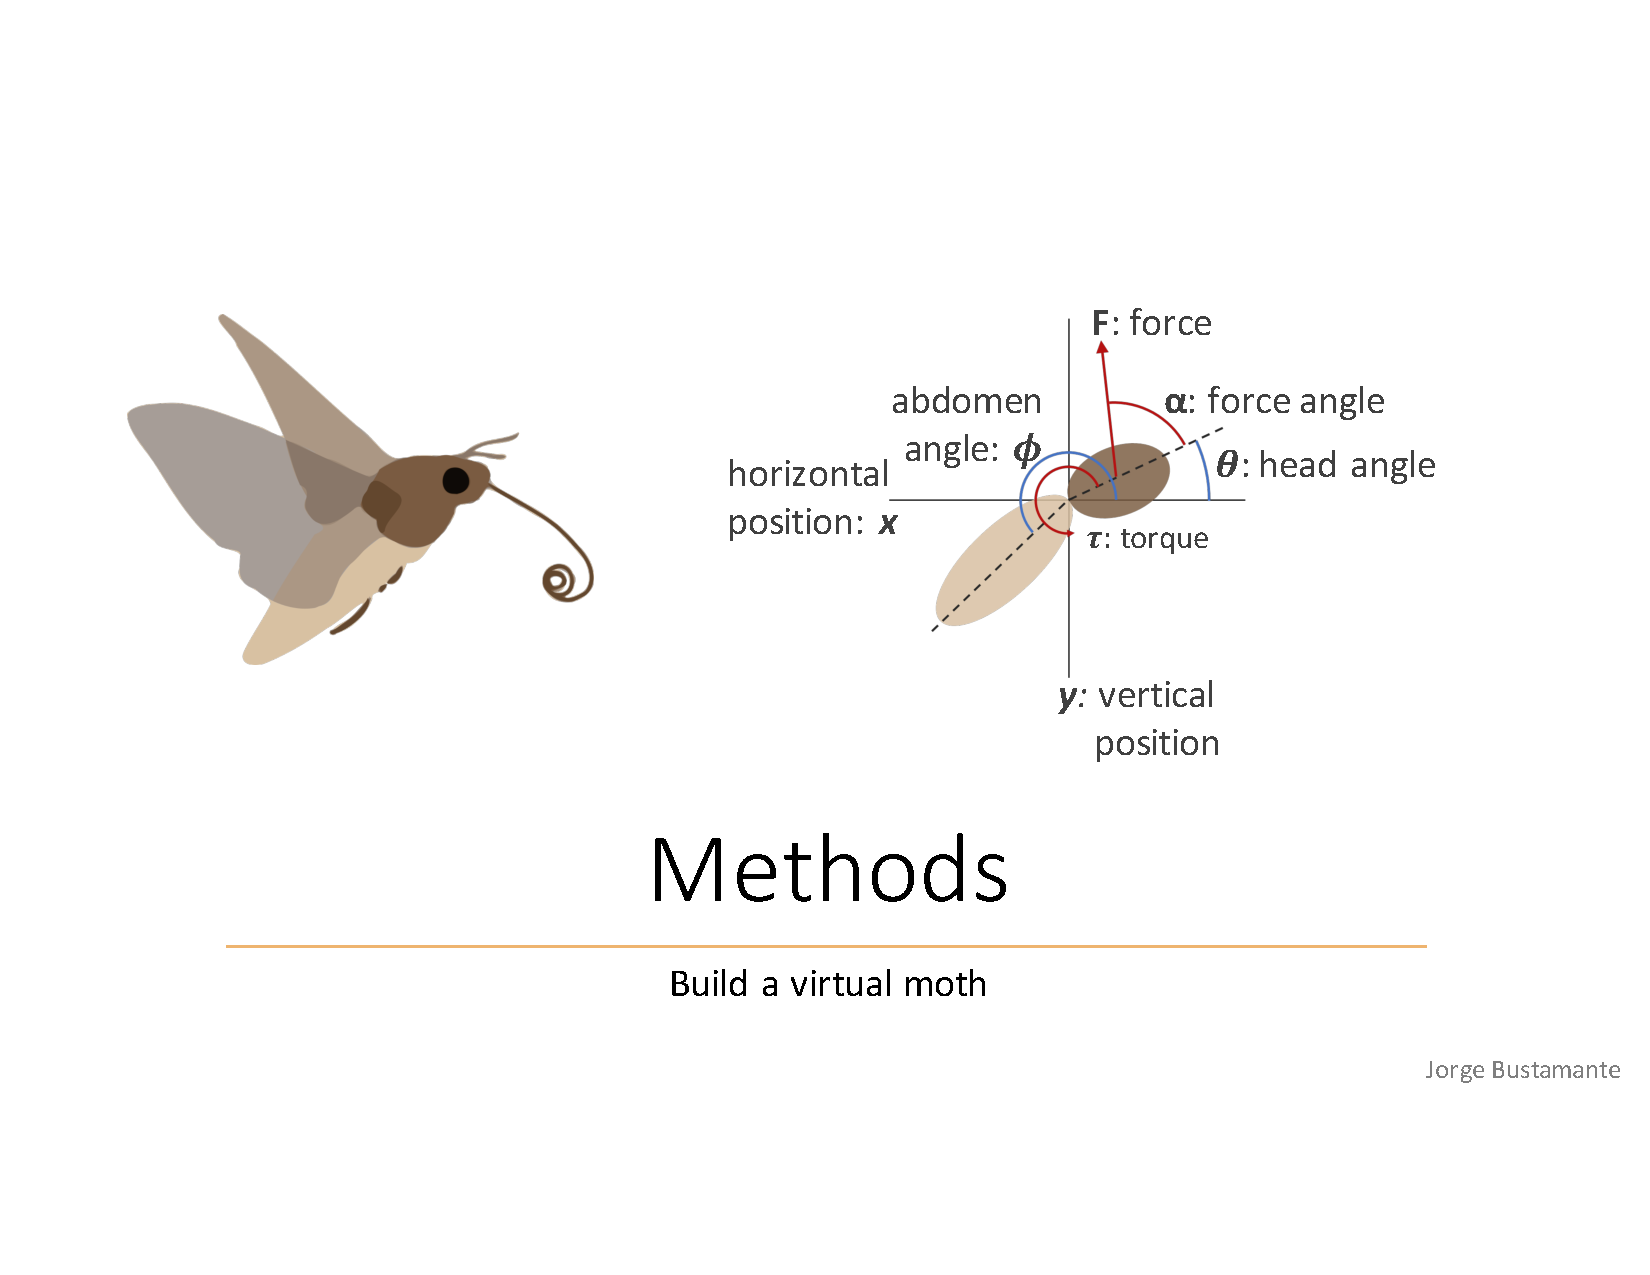
\includegraphics[scale=0.9]{s1.pdf}
  \end{center}         
   \textbf{ML Model}: Imagine a moth trying to fly, it knows its current position and state, and where it wants to go. To achieve the goal, it needs to figure out the force control over its body that takes it on the trajectory to the destination, ending up with some final velocity. To build a virtual moth, the following types of feedforward neural networks were designed, going from "where I am" and "where I want to go" (inputs), to the corresponding controls and final derivatives (outputs).
\begin{center}
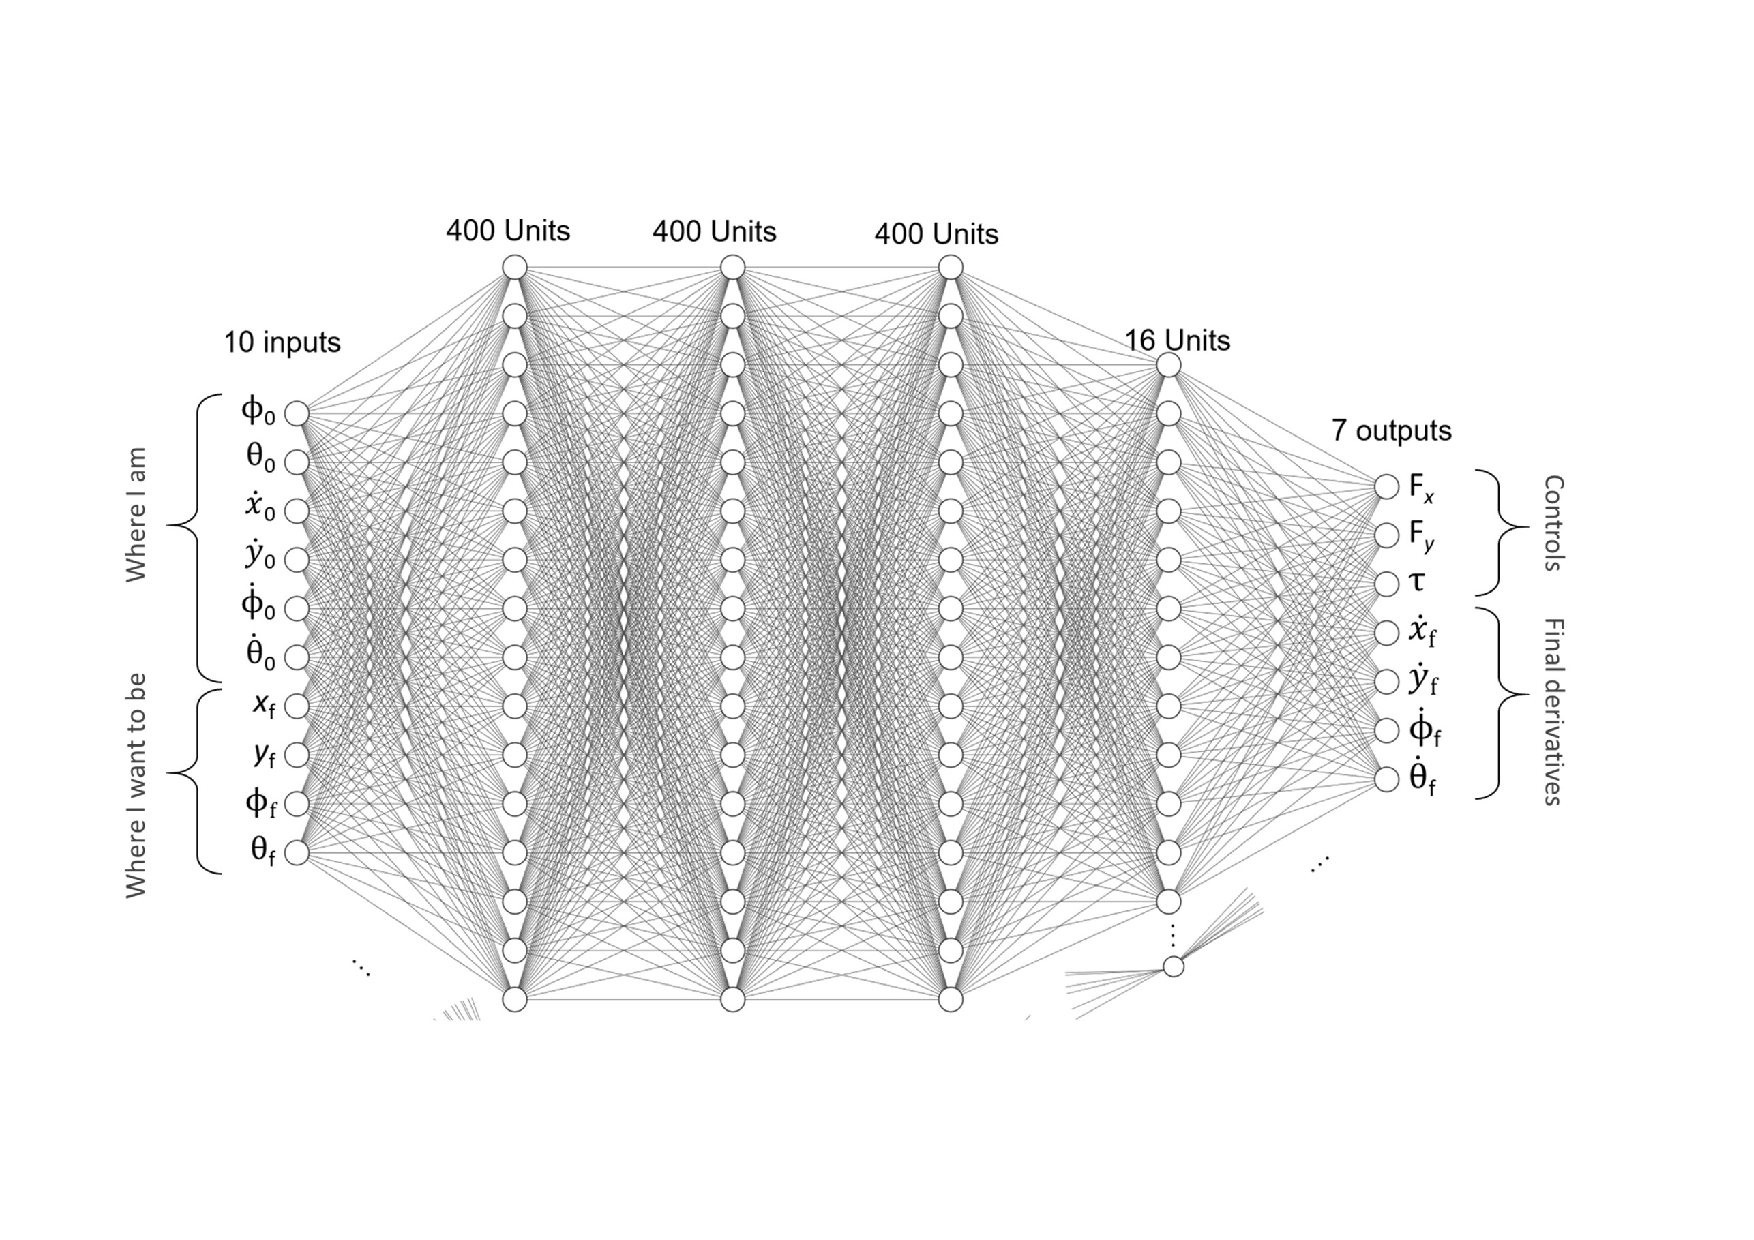
\includegraphics[scale=1]{s2.pdf}
\end{center}         
\textbf{Goal and Challenges}:  \\

1. Visualize the architecture of trained neural networks with different structures. \\

2. Interactively show the activities in the neural networks in various scenarios. \\
\bigskip

\begin{itemize}
\item For a highly pruned network, how to visualize the efficient connections in it? For a non-pruned network, how to highlight the dominant structures that may give intuitions for further training?

\item How to accommodate to network structures from a small one with less than 100 nodes to a huge network with over 2000 of nodes and about 800000 edges? 

\item How to visualize the interconnected activities of the nodes, and highlight the active parts for a certain movement?

\bigskip
\bigskip
\bigskip
\bigskip

\end{itemize}
   \end{block}

    \vfill
   \end{column}

      \begin{column}{.4\linewidth}
      \begin{block}{Visualizing Neural Network Architectures}
      \noindent The following is a small pruned neural network with $3$ hidden layers of sizes: $20,\ 20,\ 16$.\\
      \noindent The inputs mimic a jumping up of the virtual moth: $x_f = 0.25, y_f = 0.5, \dot{x}_0 = 0.5, \dot{y}_0 = 0, \phi_0=-0.25, \theta_0=0.25, \phi_f=-0.15, \theta_f=0, \dot{\phi}_0 = -0.5, \dot{\theta}_0 = 0.5$. \\
      \bigskip
      The brushing bar at the bottom selects connections with absolute weights in a desired range. The thickness and opacity of the edges shows the absolute values of the weights. The size of the nodes show the values after activation. The colors of the edges and nodes represent the signs of the values. In the following display, only weights with absolute values greater than 1 are shown, and we can see the major information flow in the network. Also, for the above input values, only certain groups of nodes are active.
      \vspace{0cm}
      \begin{center}
                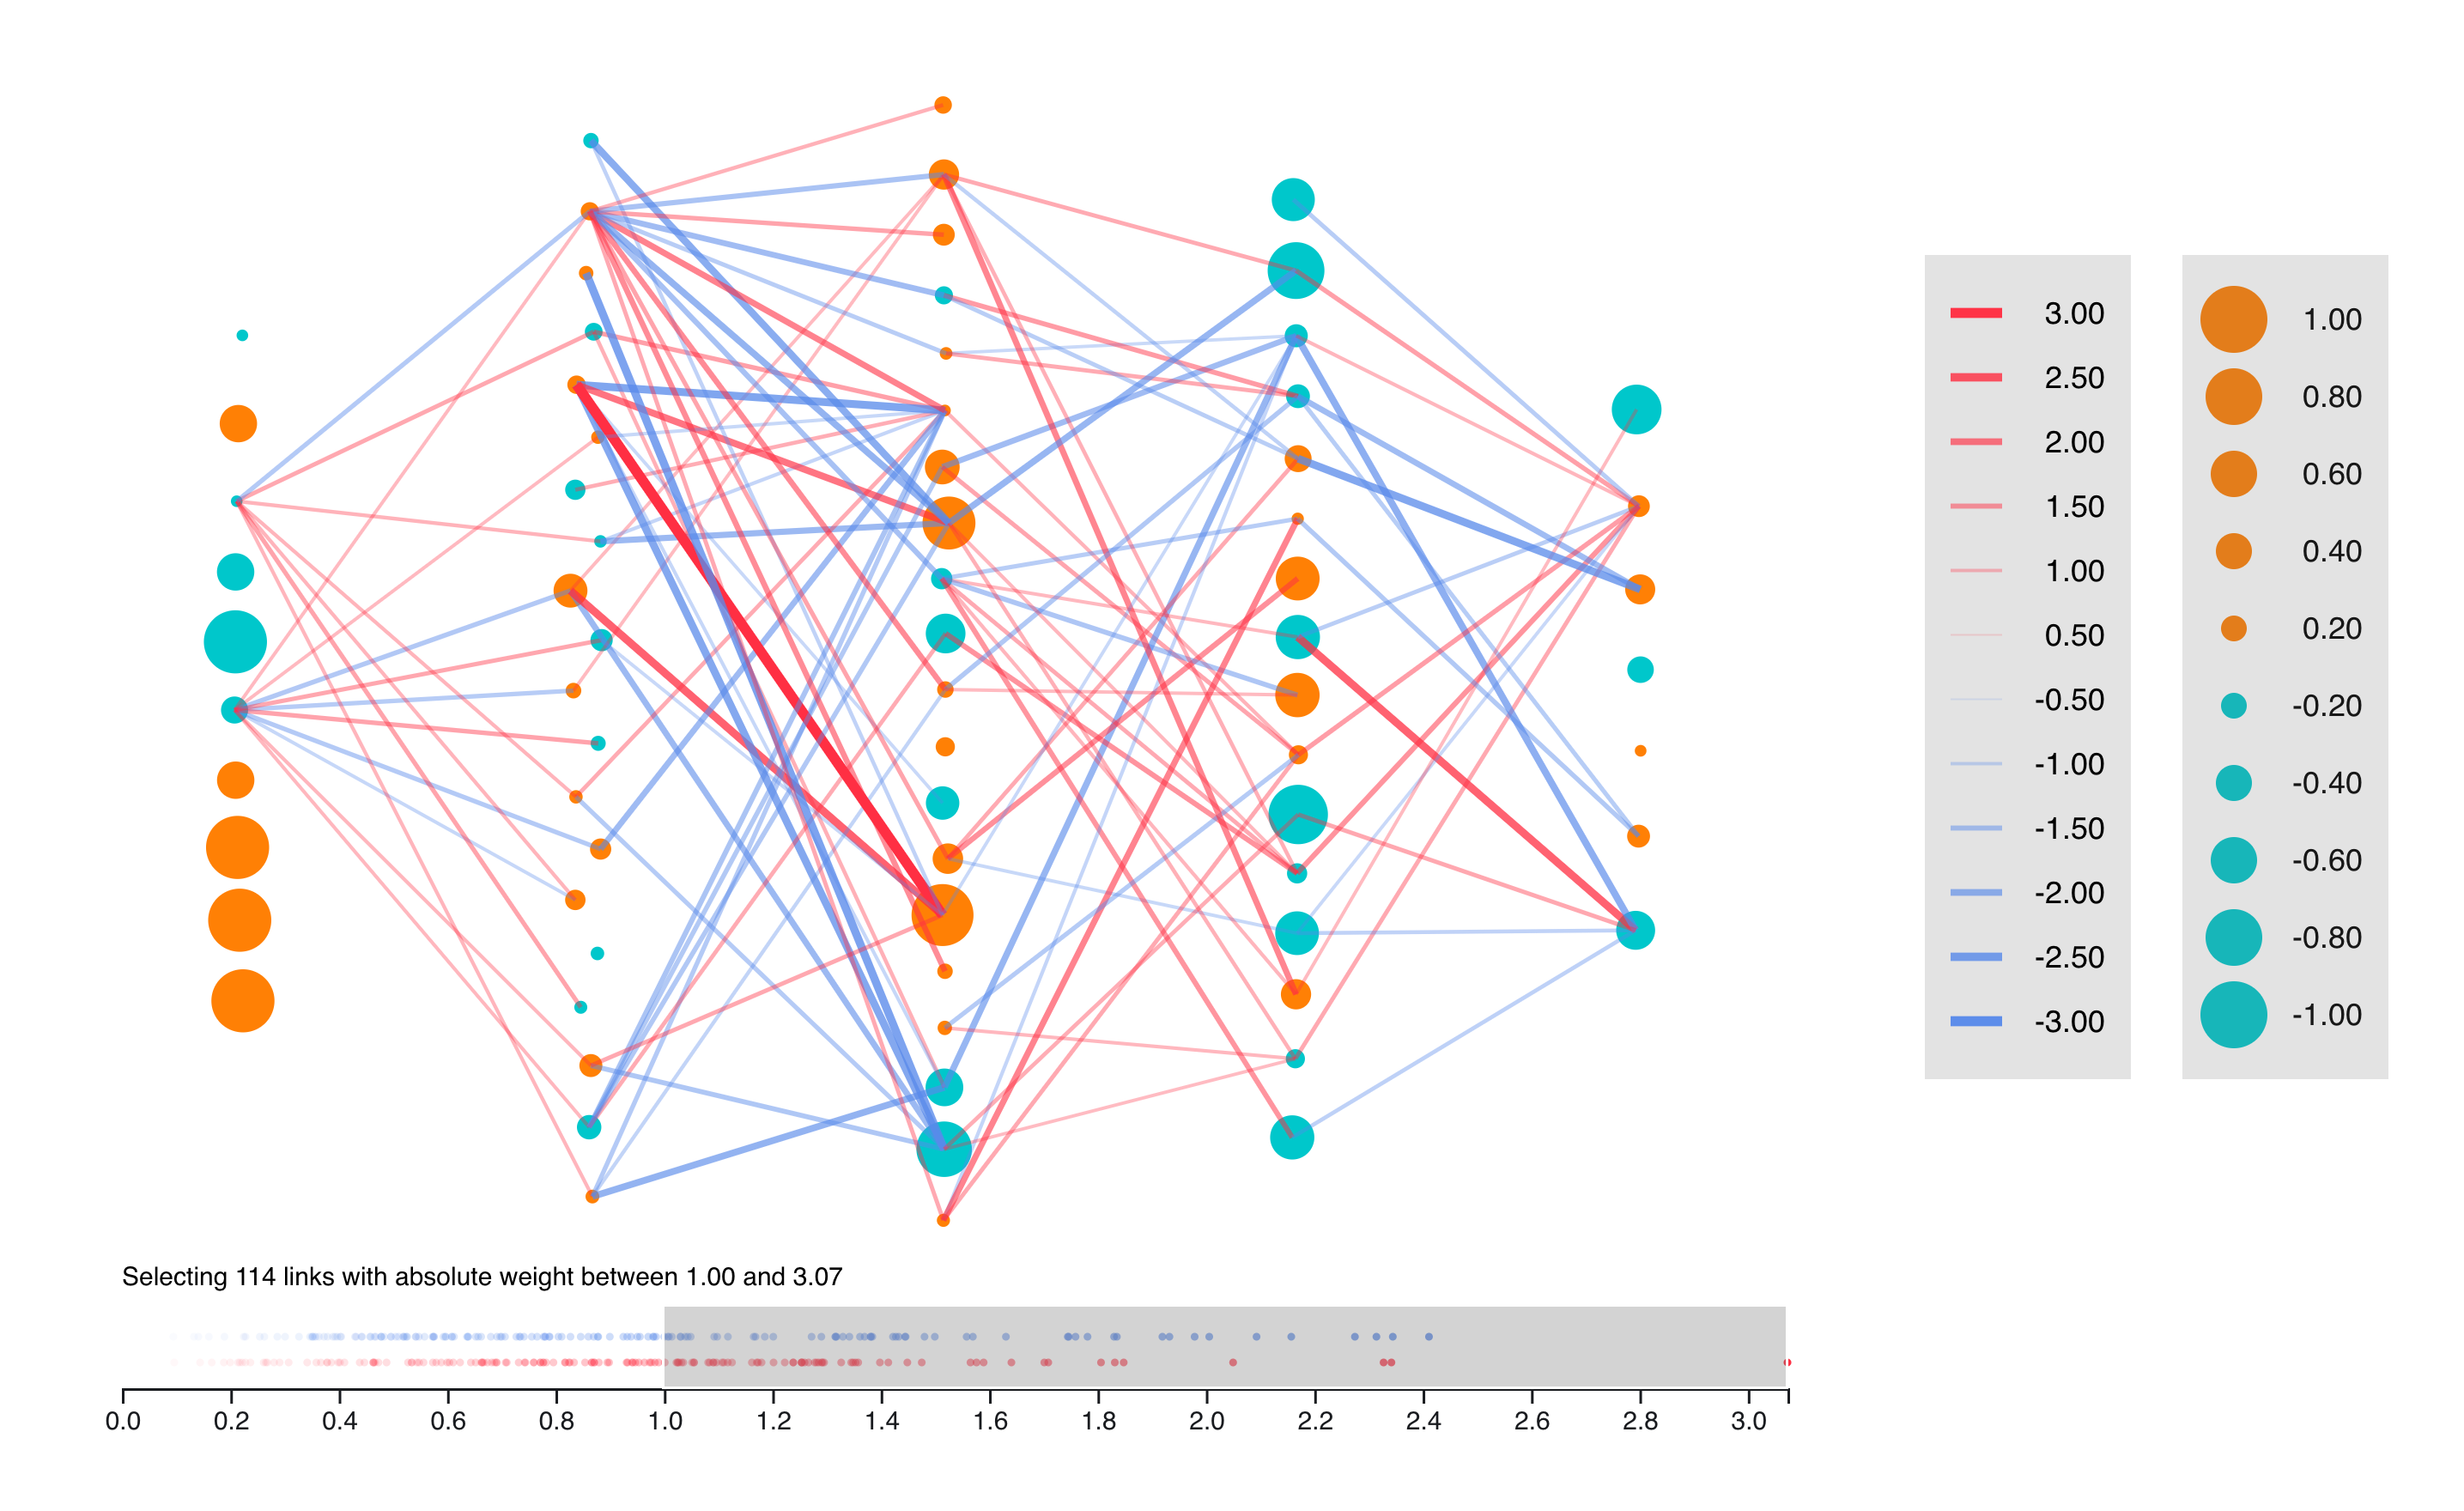
\includegraphics[scale=0.7]{NN.png}
      \end{center}
      \vspace{1cm}
        \noindent The following is a large pruned neural network with $4$ hidden layers of sizes: $512,\ 512,\ 512,\ 512$.\\
      The inputs mimic a simple forward speeding up movement: final destination $x_f = 0.5$, and all other initial states are at rest: $y_f = \dot{x}_0 =  \dot{y}_0 = \phi_0= \theta_0= \phi_f= \theta_f= \dot{\phi}_0 =  \dot{\theta}_0 = 0$. \\
      \bigskip
      To tackle the challenge of visualizing a huge network with over 2000 nodes in a relatively small space that is easy to view, we chose the force directed layout scheme, which clusters nodes on different layers into several "disks". The other challenge at the price of that is the expensive computation of the forces between 2000 nodes and 800000 links. To deal with that, we trimmed out edges with nearly zero weights, and then throw out nodes that aren't effectively connected with other nodes. The size of the network is largely reduced after this trimming, and the network plotting becomes possible.
       \vspace{0cm}
       \begin{center}
                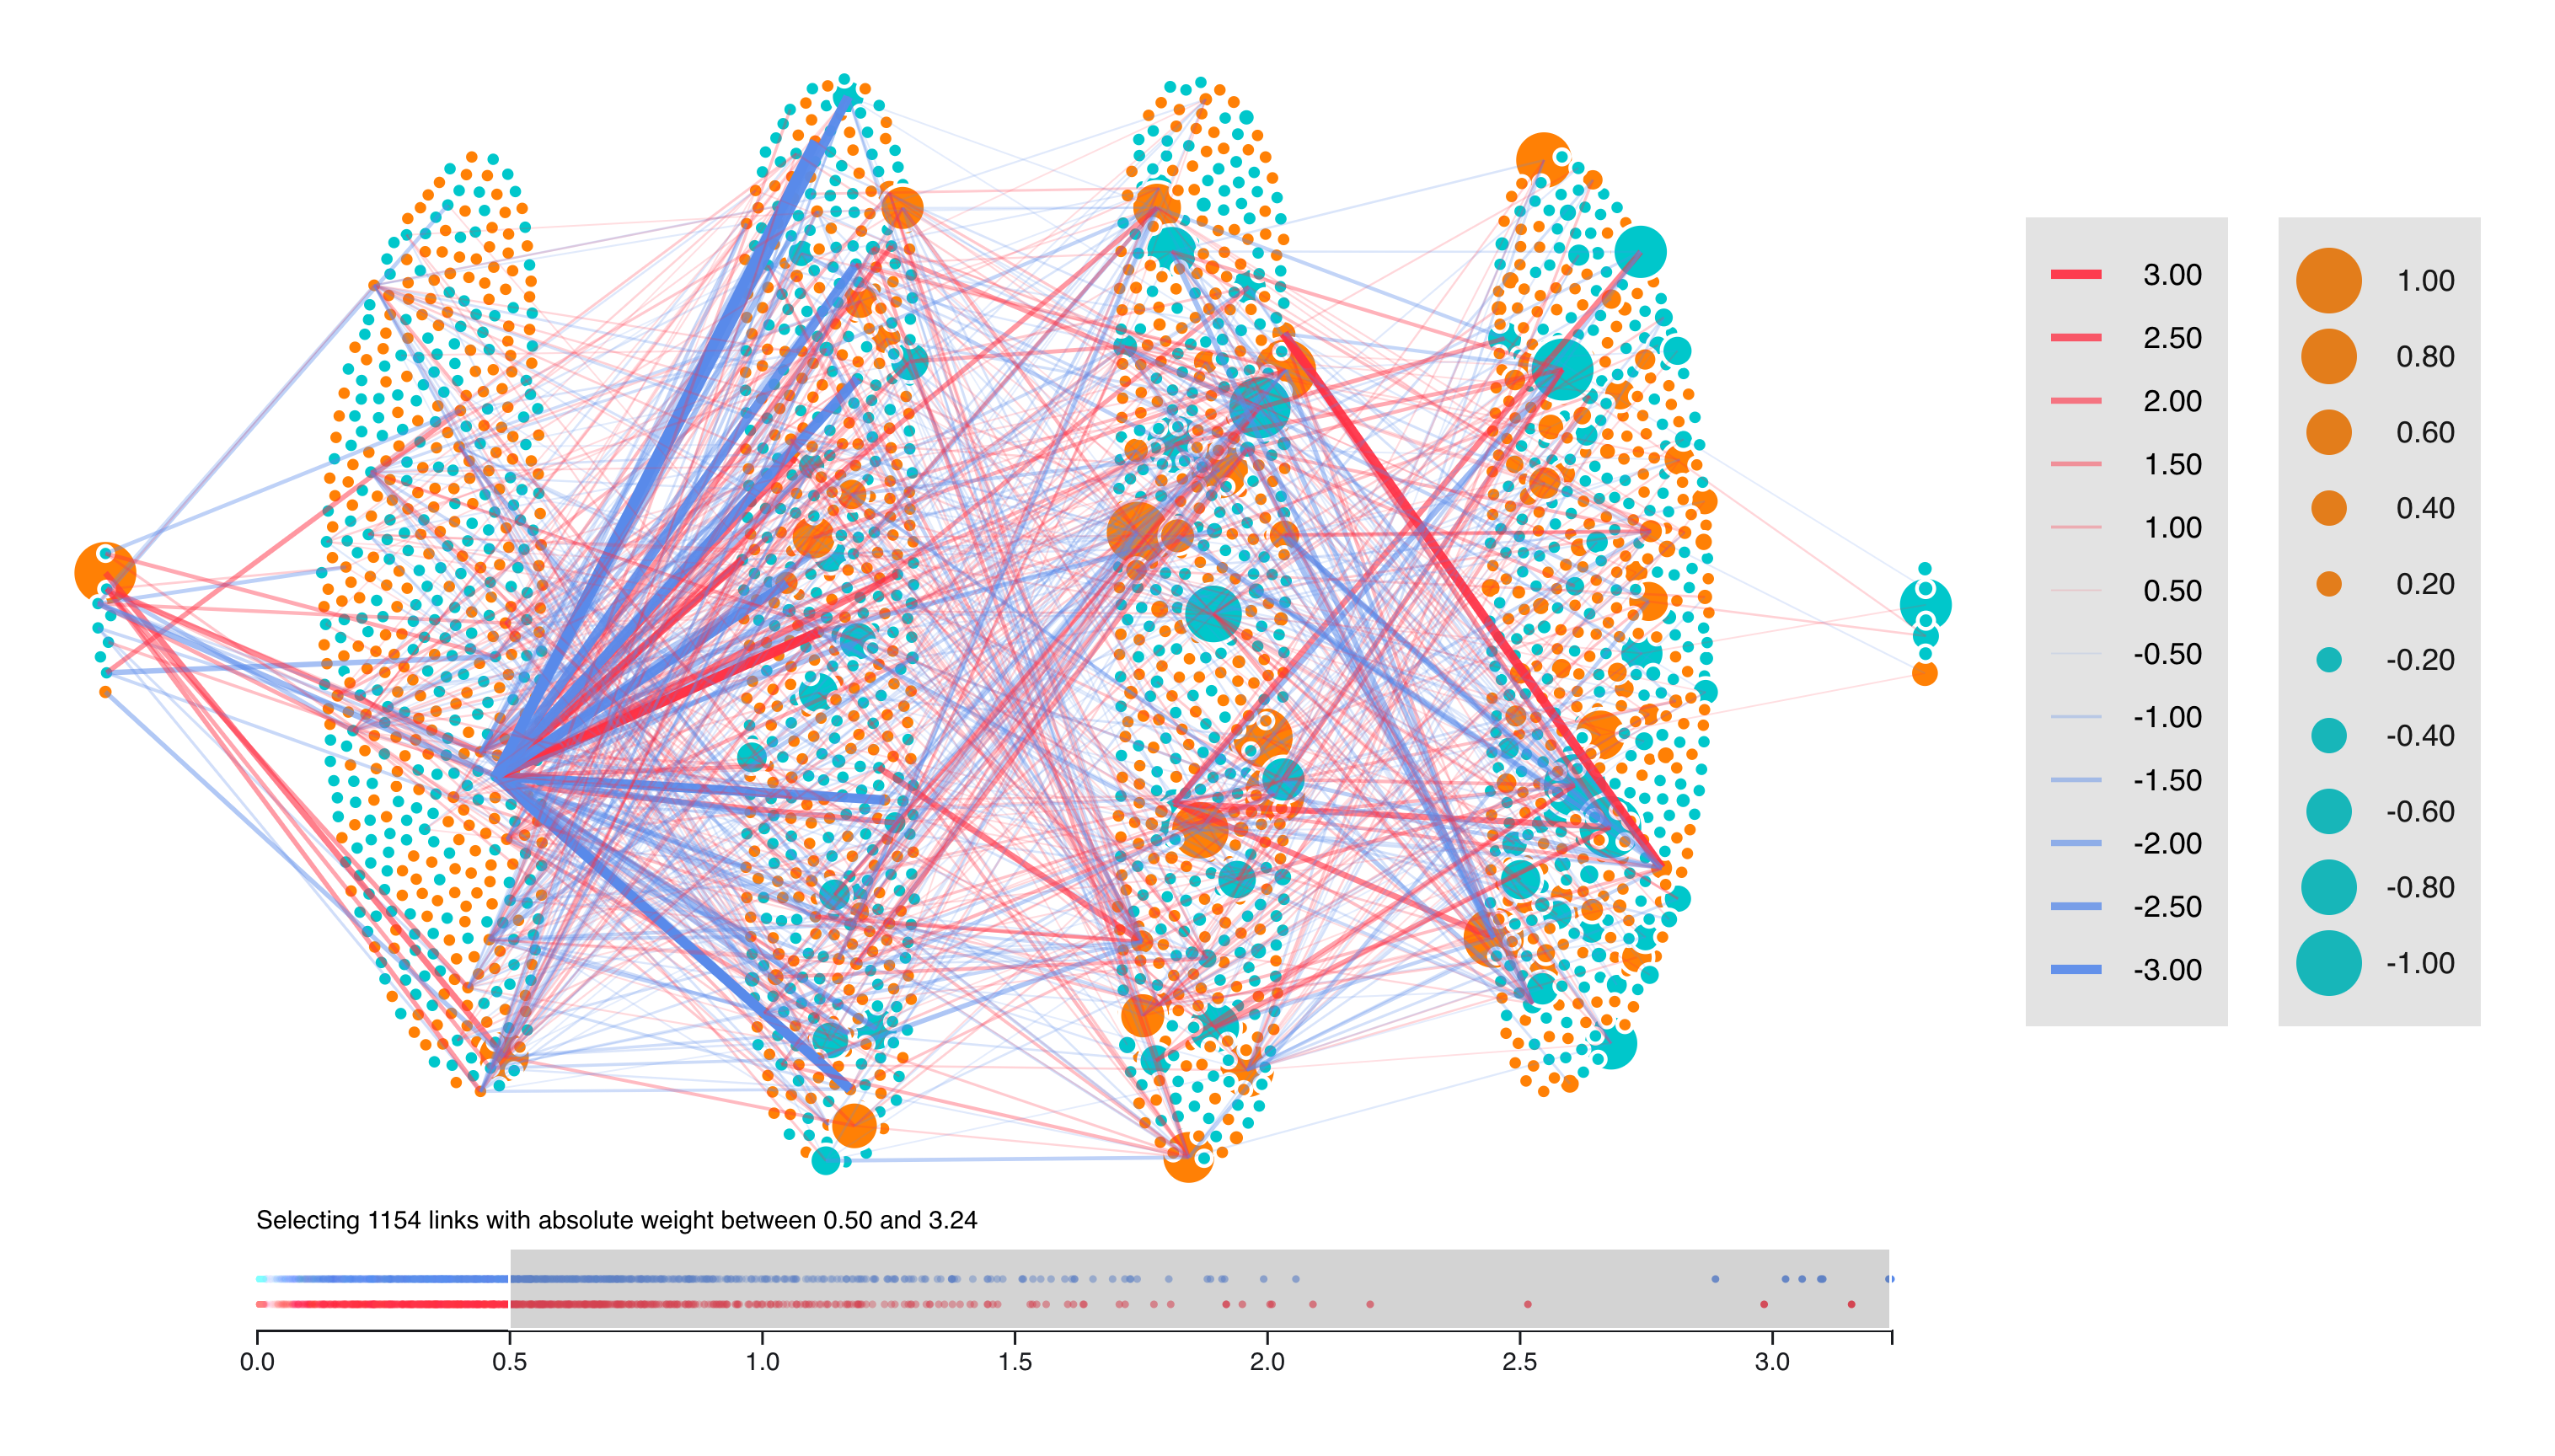
\includegraphics[scale=0.7]{NNmax1.png}
      \end{center}
      \vspace{3cm}
      \end{block}
      \end{column}
      
\begin{column}{.3\linewidth}
\begin{block}{Interaction of the Computational Graph}
The key feature of the visualization system for virtual moth neural networks is that it implements the computational graph interactively. At the heart of the system behind the visualization is forward pass algorithm that computes the values in the layers in real-time. The following slide bars allows users to choose any customized input values in a certain range from $-0.5$ to $0.5$. \\
\vspace{0cm}
      \begin{center}
                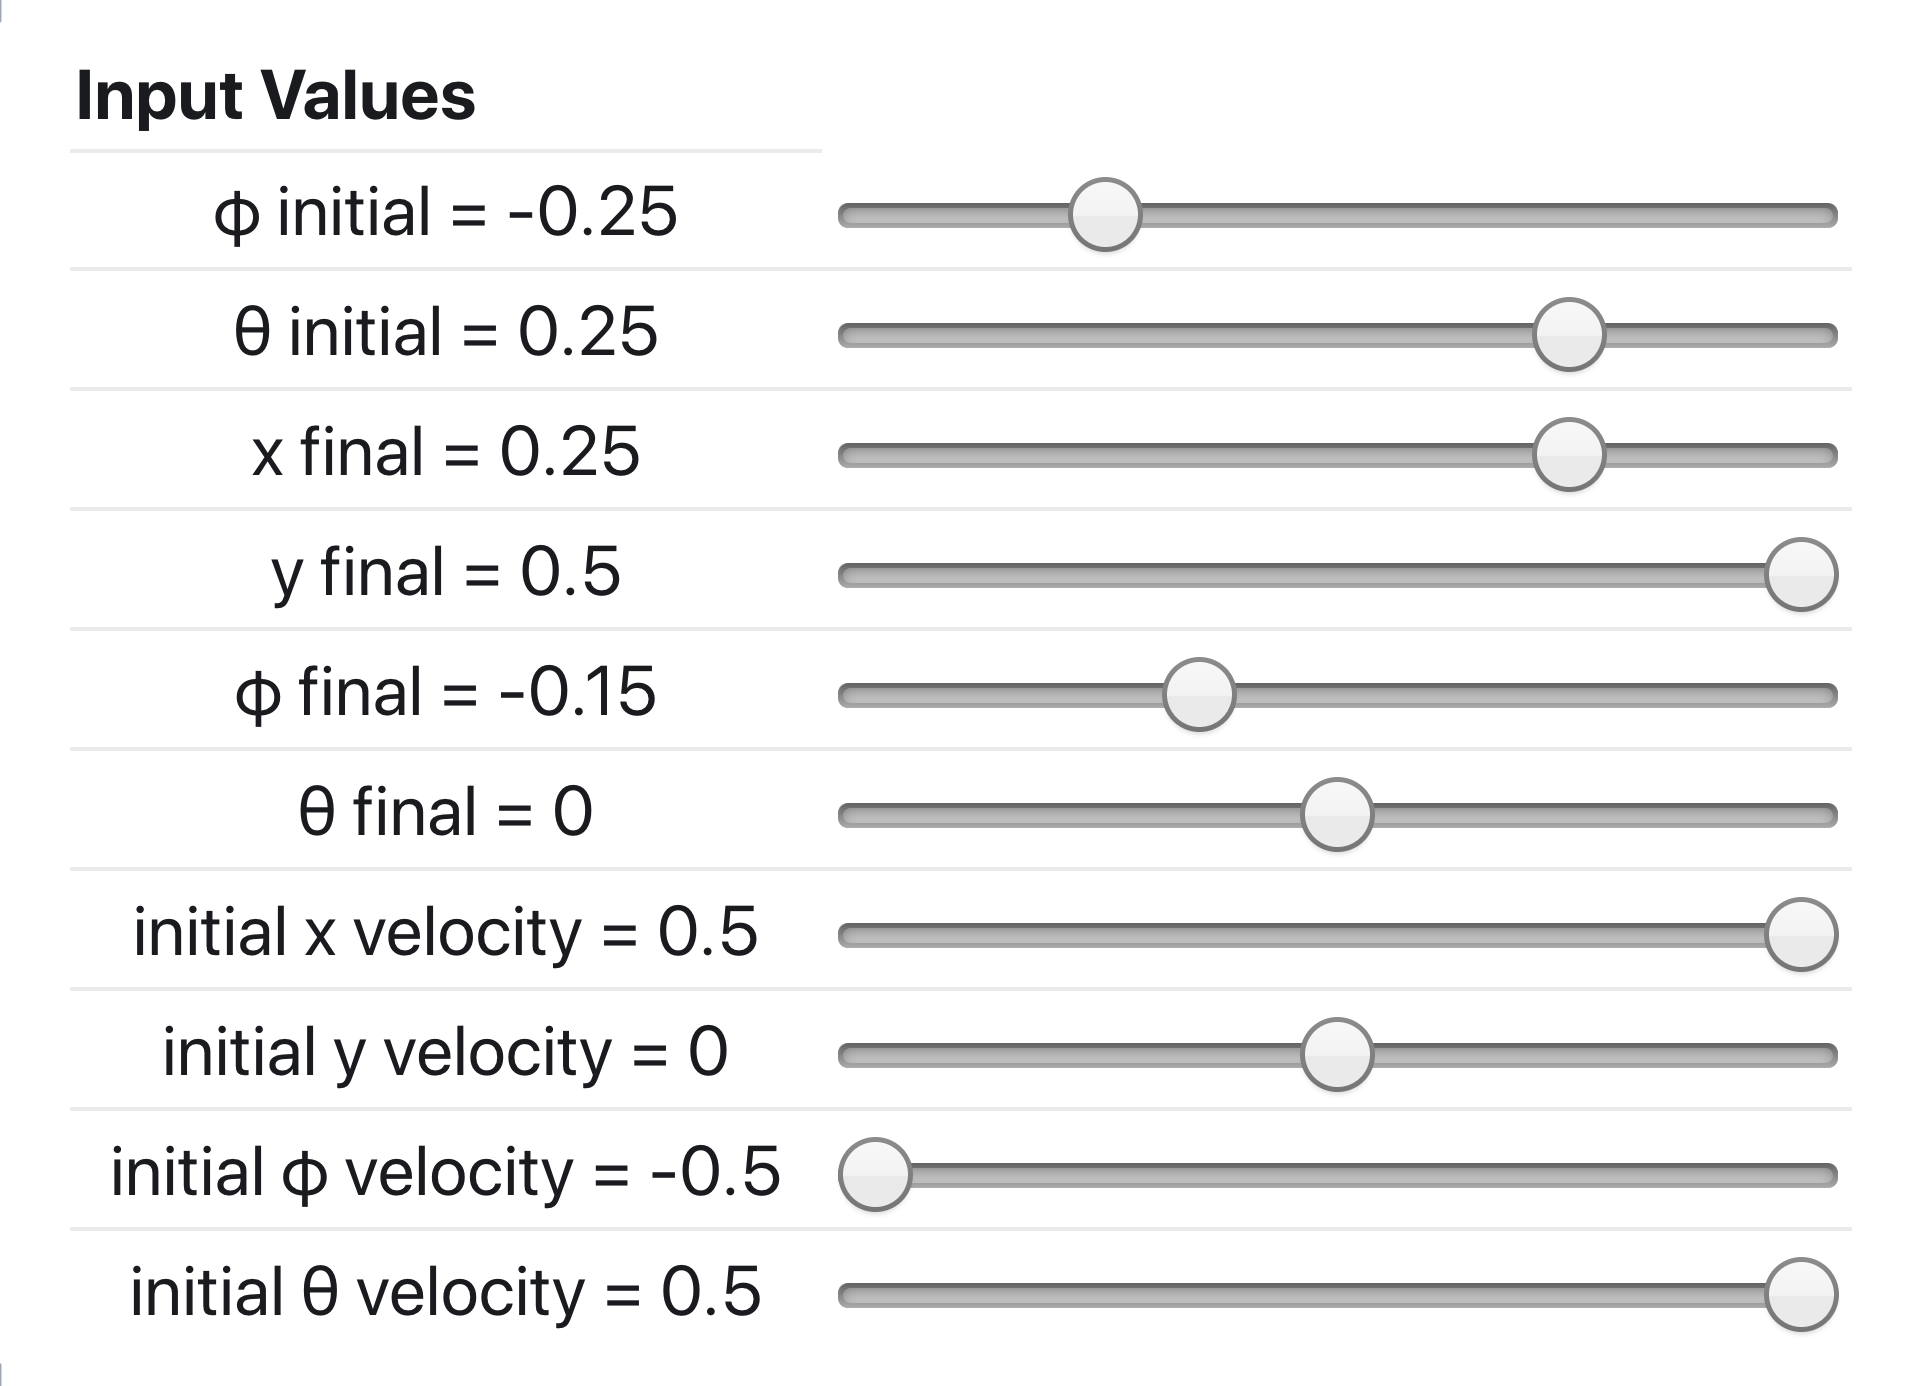
\includegraphics[scale=0.5]{slider.png}
      \end{center}
      \vspace{1cm}

Besides real-time input adjustment with the sliders, below are other useful interaction help the user to identify interesting information in the network: 
\bigskip
\begin{itemize}
\item The nodes can be dragged to re-position in the force directed way. Since all the nodes in one hidden layer are essentially identical, we can wisely choose their positions such that the links to the next layer are shown clearer.

\item The brush allows for choosing the range of the absolute weights to be shown, which is useful for users to see the dominant weights and the effect of network pruning. 
\end{itemize}
\vspace{0cm}
      \begin{center}
                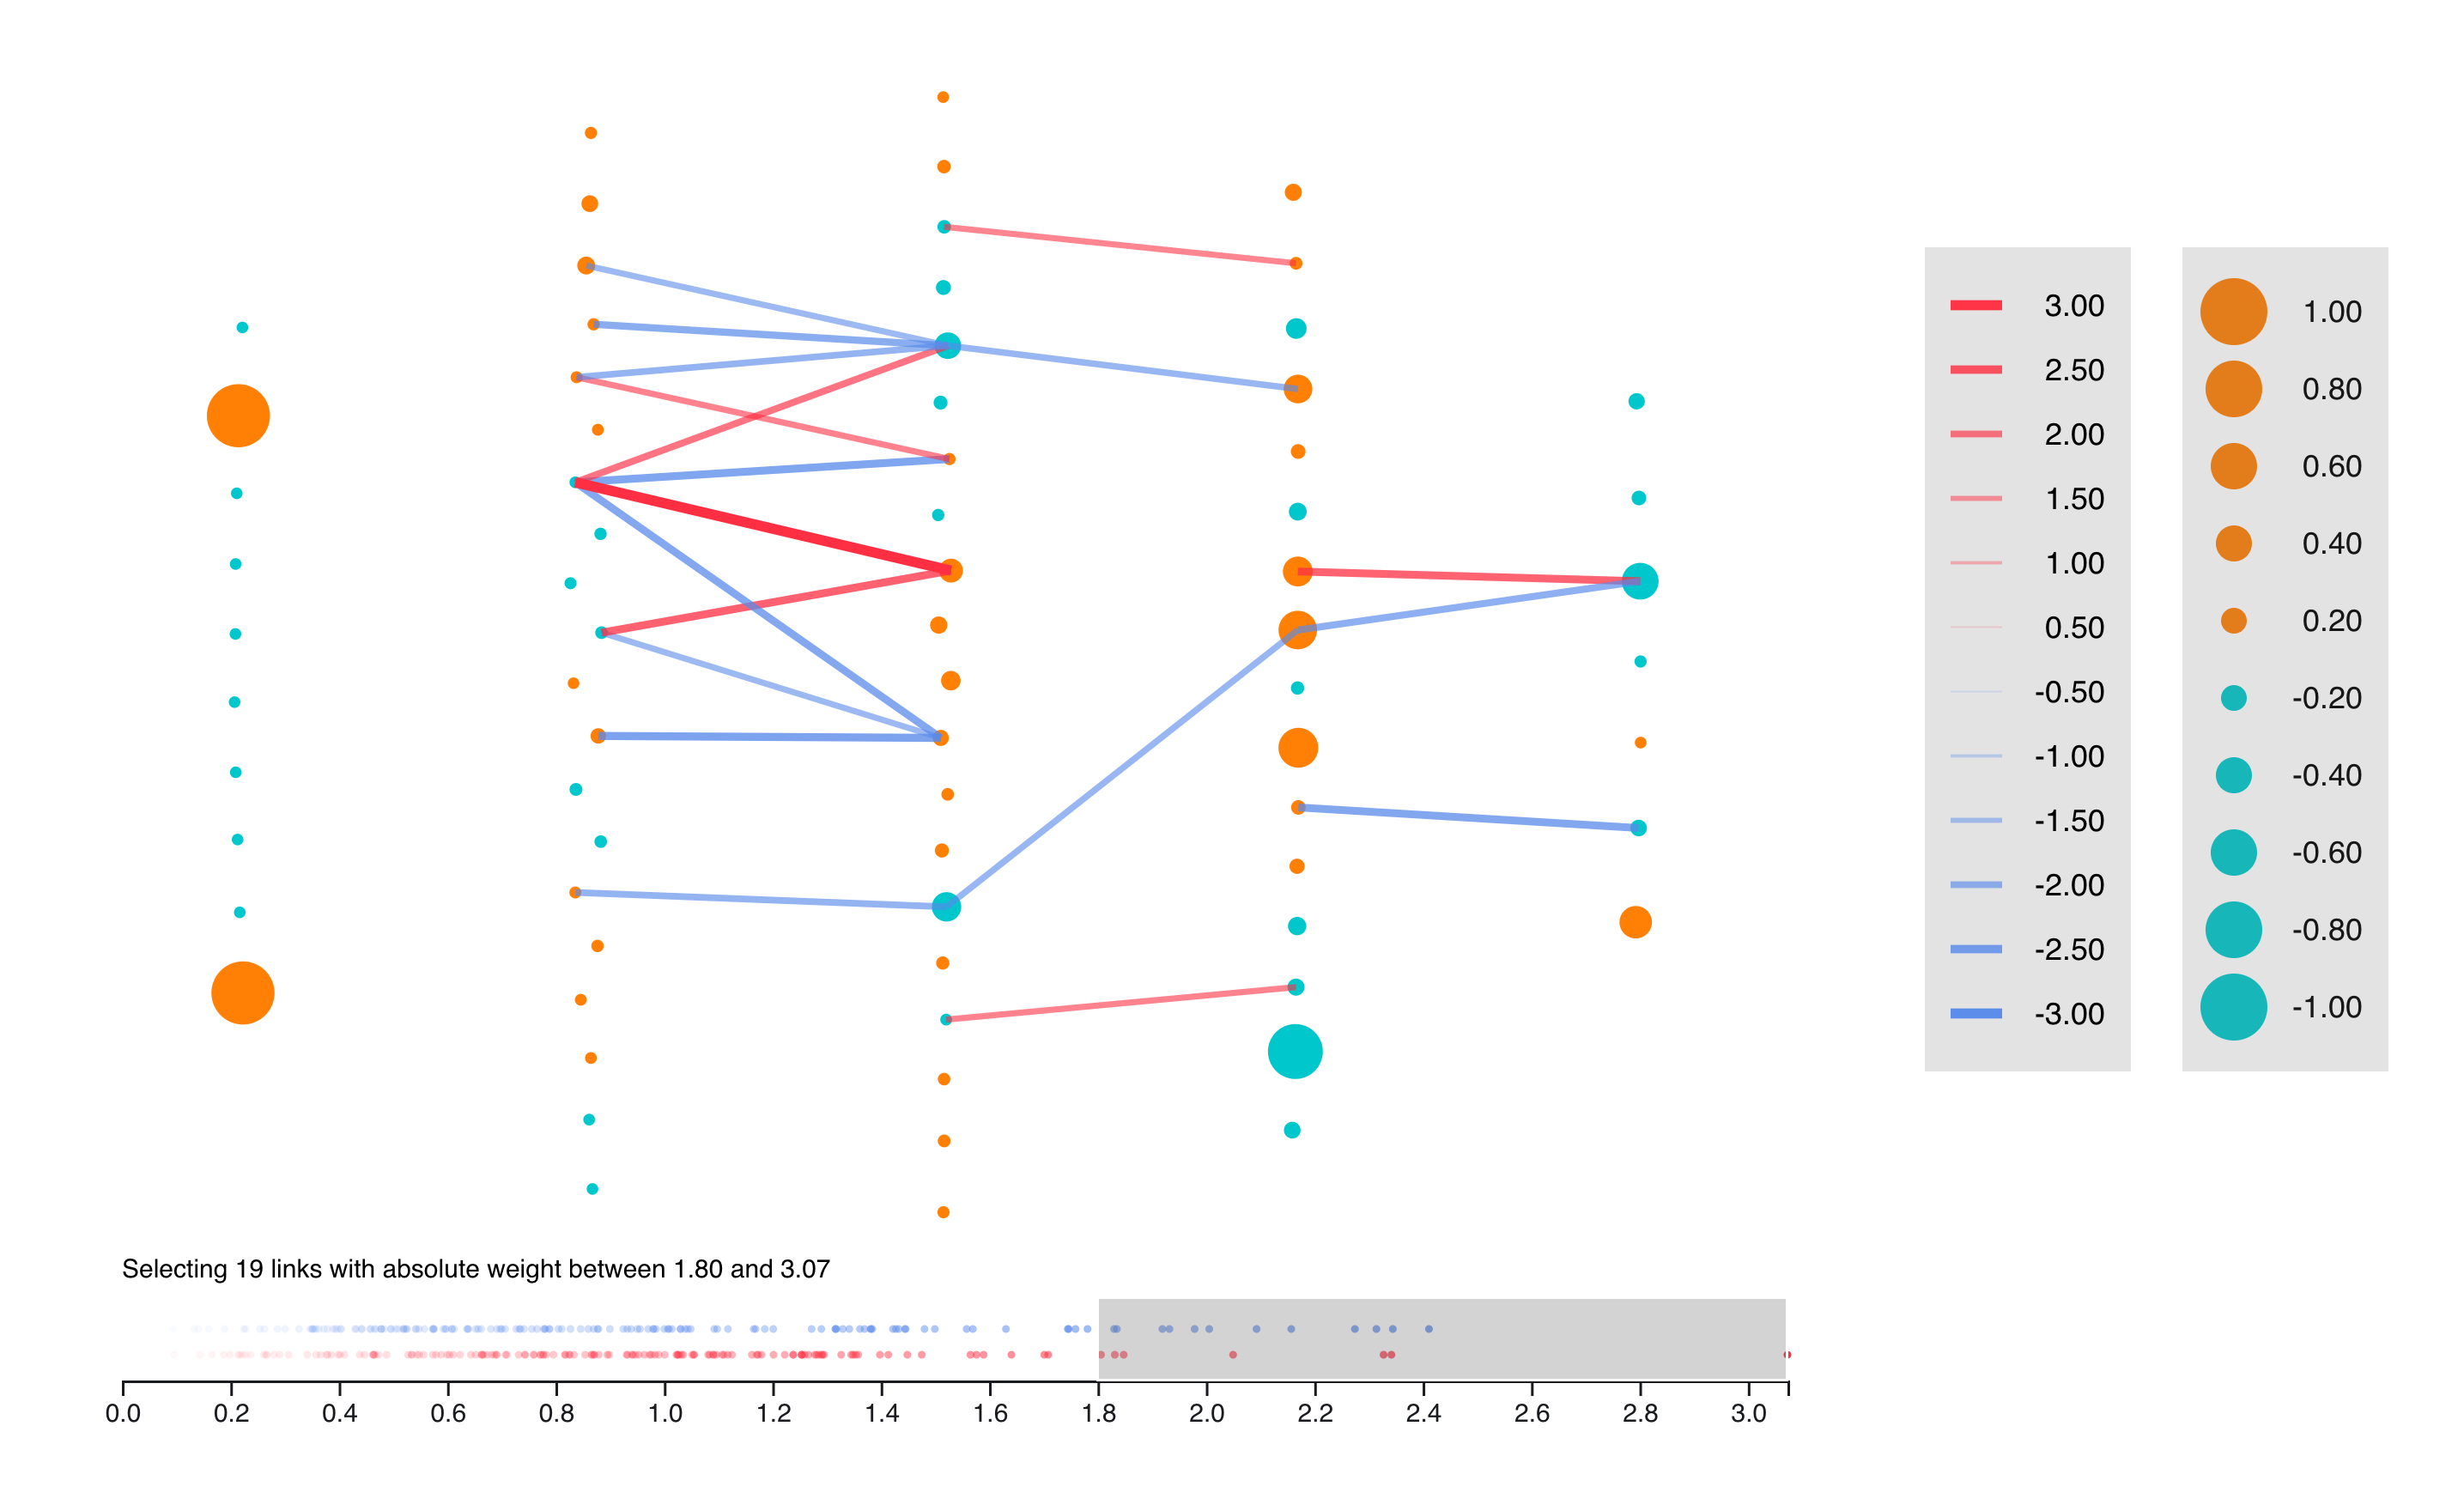
\includegraphics[scale=0.5]{NNinter.png}
      \end{center}
      \vspace{0cm}
Above is the same small neural network, after the above described interaction. The slide bar changes the input to a simple forward flying with $x_f = \dot{x}_0 = 0.5$, and all other values are zeros. Rearranging the nodes and filter only the weights with absolute values greater than 1.8, we see a much cleaner network and can figure out how are the nodes connected between layers with the largest strength.
\end{block}   

\begin{block}{Future Improvements}
Besides the current features, there can be additional improvements in future work.
\begin{itemize}
\item Hide all "dead'' nodes which are not active in real time.
\item For each node, show the strongest path that is connected with it.
\item Show the activity level of each edge as well, activated by the outcoming node. 
\item Visualize the configuration of the virtual moth in real-time, which helps the audience to understand the meaning of the inputs and outputs better. 
\item Visualize the distribution of the nodes values in real-time, as an estimation of "neuron activity level".
\end{itemize}
\bigskip
\bigskip
\end{block}   

      
      \end{column}

      
    \end{columns}
  \end{frame}
\end{document}


%%%%%%%%%%%%%%%%%%%%%%%%%%%%%%%%%%%%%%%%%%%%%%%%%%%%%%%%%%%%%%%%%%%%%%%%%%%%%%%%%%%%%%%%%%%%%%%%%%%%
%%% Local Variables:
%%% mode: latex
%%% TeX-PDF-mode: t
%%% End:
